\chapter{Подсистема Экосистемы OSTIS, обеспечивающая поддержку жизненного цикла интеллектуальных геоинформационных систем различного назначения}
\chapauthortoc{Самодумкин С.~А.\\Зотов Н.~В.}
\label{chapter_gis}

\vspace{-7\baselineskip}

\begin{SCn}
\begin{scnrelfromlist}{авторы}
	\scnitem{Самодумкин С.~А.}
	\scnitem{Зотов Н.~В.}
\end{scnrelfromlist}

\bigskip
	
\scntext{аннотация}{Глава посвящена частной технологии проектирования \textit{интеллектуальных геоинформационных систем}, построенных по принципам \textit{Технологии OSTIS}. \textit{интероперабельность} \textit{геоинформационных систем}, построенных по предлагаемой технологии, обеспечивается за счет перехода от карты к семантическому описанию элементов карты.}

\bigskip

\begin{scnrelfromlist}{подраздел}
	\scnitem{\ref{chapter_gis_sec_requirements}~\nameref{chapter_gis_sec_requirements}}
	\scnitem{\ref{chapter_gis_sec_tasks}~\nameref{chapter_gis_sec_tasks}}
	\scnitem{\ref{chapter_gis_sec_components}~\nameref{chapter_gis_sec_components}}
	\scnitem{\ref{chapter_gis_ps}~\nameref{chapter_gis_ps}}
	\scnitem{\ref{chapter_gis_sec_map_specification}~\nameref{chapter_gis_sec_map_specification}}
	\scnitem{\ref{chapter_gis_sec_mic_components}~\nameref{chapter_gis_sec_mic_components}}
	\scnitem{\ref{chapter_gis_sec_automatization}~\nameref{chapter_gis_sec_automatization}}
\end{scnrelfromlist}

\bigskip

\begin{scnrelfromlist}{ключевое понятие}
	\scnitem{геоинформационная система}
	\scnitem{интеллектуальная геоинформационная система}
	\scnitem{задача геоинформационной системы}
	\scnitem{интеллектуальная геоинформационная ostis-система}
	\scnitem{база знаний интеллектуальной геоинформационной ostis-системы}
	\scnitem{геоонтология}
	\scnitem{объект местности}
	\scnitem{геосемантическая характеристика объекта местности}
	\scnitem{пространственное отношение}
	\scnitem{решатель задач интеллектуальной геоинформационной ostis-системы}
	\scnitem{картографический интерфейс}
	\scnitem{картографический интерфейс интеллектуальной геоинформационной ostis-системы}
\end{scnrelfromlist}

\begin{scnrelfromlist}{ключевой параметр}
	\scnitem{класс объектов местности\scnsupergroupsign}
\end{scnrelfromlist}

\begin{scnrelfromlist}{ключевой знак}
	\scnitem{Технология проектирования интеллектуальных геоинформационных систем}
	\scnitem{Язык карт для ostis-систем}
\end{scnrelfromlist}

\bigskip

\begin{scnrelfromlist}{библиографическая ссылка}
	\scnitem{\scncite{Ablameiko2000}}
	\scnitem{\scncite{Batalov2021}}
	\scnitem{\scncite{Beliakova2016}}
	\scnitem{\scncite{Berezko2009}}
	\scnitem{\scncite{Bliskavitskiy2012}}
	\scnitem{\scncite{Bliskavitskiy2014}}
	\scnitem{\scncite{Zuravkov2004}}
	\scnitem{\scncite{Glotov2014a}}
	\scnitem{\scncite{Glotov2014b}}
	\scnitem{\scncite{Hubarevich2017}}
	\scnitem{\scncite{Hubarevich2018}}
	\scnitem{\scncite{Ivakin2009a}}
	\scnitem{\scncite{Dulin2016}}
	\scnitem{\scncite{Kikot2020}}
	\scnitem{\scncite{Kruchkov2006}}
	\scnitem{\scncite{Kuznetsov2012}}
	\scnitem{\scncite{Orehova2013}}
	\scnitem{\scncite{Samodumkin2011}}
	\scnitem{\scncite{Samodumkin2012}}
	\scnitem{\scncite{Samodumkin2012a}}
	\scnitem{\scncite{Samodumkin2019}}
	\scnitem{\scncite{Samodumkin2022}}
	\scnitem{\scncite{SOATO}}
	\scnitem{\scncite{Sokolov2012}}
	\scnitem{\scncite{Ataeva2011}}
	\scnitem{\scncite{Shpakov2004}}
	\scnitem{\scncite{Okrb012-2007}}
	\scnitem{\scncite{Hu2018}}
	\scnitem{\scncite{Janowicz2012}}
	\scnitem{\scncite{Yankelevich2019}}
\end{scnrelfromlist}
\end{SCn}

\section*{Введение в Главу \ref{chapter_gis}}

Современные программно-технологические комплексы \textit{геоинформационных систем} очень эффективны, но сложны в освоении и применении, поэтому требуют специальной профессиональной подготовки конечных пользователей. Для внедрения систем геопространственного назначения в различные области знаний и сферы применения необходимо, чтобы специалисты различного вида деятельности без особых сложностей и дополнительного обучения могли решать характерные для \textit{геоинформационных систем} задачи. Для этого необходим \myuline{переход от традиционных геоинформационных систем к геоинформационным системам нового поколения}, имеющим удобный \textit{пользовательский интерфейс}.

Целью данной главы является создание комплексной технологии проектирования интеллектуальных геоинформационных систем нового поколения по принципам, лежащим в основе \textit{Технологии OSTIS}.

\section{Требования, предъявляемые к интеллектуальным геоинформационным системам нового поколения}
\label{chapter_gis_sec_requirements}

Согласно общепринятому определению \textit{геоинформационная система} --- \textit{программная компьютерная система}, обеспечивающая ввод, манипулирование, анализ и вывод пространственно-соотнесенных данных (геоданных) о территории, социальных и природных явлениях при решении задач, связанных с инвентаризацией, анализом, моделированием, прогнозированием и управлением окружающей средой и территориальной организацией общества (см. \scncite{Kruchkov2006}).

Следовательно, из самого определение \textit{геоинформационной системы} вытекает необходимость реализации интеллектуальных задач.

\begin{SCn}
\scnheader{задача геоинформационной системы}
\begin{scnrelfromset}{разбиение}
	\scnitem{задача анализа в геоинформационной системе}
	\scnitem{задача моделирования в геоинформационной системе}
	\scnitem{задача прогнозирования в геоинформационной системе}
	\scnitem{задача управления в геоинформационной системе}
\end{scnrelfromset}
\end{SCn}

Все указанные задачи являются интеллектуальными и требуют поддержки принятия решения при их реализации.

В отличие от других классов \textit{информационных систем}, в \textit{геоинформационных системах} основным объектом исследования являются знания и данные об \textit{объектах местности}, которые рассматриваются не только как пространственные данные и знания, но и являются интеграционной основой для различных \textit{предметных областей}. При этом формализация таких \textit{знаний} и их представление в \textit{базах знаний} \textit{интеллектуальных систем} требует установления отношений для описания свойств и закономерностей, присущих рассматриваемой \textit{предметной области} и использующей \textit{объекты местности}, установления геометрических характеристик, способных осуществить привязку \textit{объектов местности}, а также учитывает темпоральный (временной) характер существование \textit{объектов местности}, что позволяет осуществить ретроспективный анализ. С учетом того, что \textit{интеллектуальные системы} предназначены для удовлетворения \textit{информационной потребности пользователей}, данный факт способствует расширению \textit{предметных областей} и добавления новых функциональных возможностей в рамках предлагаемой частной \textit{Технологии проектирования интеллектуальных геоинформационных систем}.

\begin{SCn}
\scnheader{интеллектуальная геоинформационная система}
\scnidtf{информационная система, основным объектом исследования которой являются знания и данные об объектах местности, выступающие интеграционной основой для решения прикладных задач в различных предметных областях}
\scnsuperset{интеллектуальная геоинформационная ostis-система}
\begin{scnindent}
	\scnsubset{ostis-система}
	\scnidtf{интеллектуальная геоинформационная система, разработанная по принципам Технологии OSTIS}
	\begin{scnrelfromset}{обобщенная декомпозиция}
		\scnitem{база знаний интеллектуальной геоинформационной ostis-системы}
		\scnitem{решатель задач интеллектуальной геоинформационной ostis-системы}
		\scnitem{картографический интерфейс интеллектуальной геоинформационной ostis-системы}
	\end{scnrelfromset}
\end{scnindent}
\end{SCn}

Важным моментом, снижающим с одной стороны срок разработки \textit{интеллектуальных систем}, а с другой --- повышающим функциональные возможности \textit{интеллектуальных систем}, использующих знания об \textit{объектах местности}, является наличие технологии проектирования таких систем. При этом \textit{Технология проектирования интеллектуальных геоинформационных систем} должна быть ориентирована на многократное использование функциональных компонентов системы с целью сокращения сроков проектирования и разработки прикладных систем. Таким образом, речь идет о создании частной \textit{Технологии проектирования интеллектуальных геоинформационных систем}. В связи среди актуальных задач можно выделить следующие: 
\begin{textitemize}
	\item проектирование пространственных онтологий и на основе их решение проблемы \textit{семантической совместимости} \textit{знаний} \textit{предметных областей};
	\item решение задачи управления метаданными и совершенствования поиска, доступа и обмена в условиях растущих объемов пространственной информации и сервисов, предоставляемых многочисленными источниками \textit{геоинформации};
	\item осуществление вывода знаний с использованием пространственной и тематической информации как составляющих \textit{знаний} \textit{объектов местности} с использованием \textit{Языка вопросов} (см. \textit{Главу \ref{chapter_requests}~\nameref{chapter_requests}});
	\item внедрение \textit{картографического интерфейса} в \textit{интеллектуальные ostis-системы} как естественного для человека способа представления информации об \textit{объектах местности}.
\end{textitemize}

Постоянная эволюция моделей и средств онтологического описания предметных областей, использующих пространственные и темпоральные компоненты, их неоднородность и неоднозначность, ставит новые задачи с точки зрения взаимодействия, интеграции и обеспечения совместимости различных прикладных систем за счет:
\begin{textitemize}
	\item интеграции \textit{предметных областей} и соответствующих им онтологий (вертикальный уровень), 
	\item расширения функциональных возможностей систем при помощи повторно используемых компонентов этих систем (горизонтальный уровень), в частности, проектирование компонентов для новых территорий или в новом временном интервале.
\end{textitemize}

С целью выполнения предъявленных требований предлагается рассматривать карту как \textit{информационную конструкцию}, элементами которой являются \textit{объекты местности}. Для этого предложены:
\begin{textitemize}
	\item \textit{Предметная область и онтология объектов местности};
	\item \textit{Спецификация Языка карт для ostis-систем};
\end{textitemize}

Переход от карт к их \textit{смыслу} осуществляется на основе:
\begin{textitemize}
	\item формального описания \textit{Синтаксиса Языка карт для ostis-систем};
	\item формального описания \textit{Денотационной семантики Языка карт для ostis-систем}.
\end{textitemize}

При этом \textit{семантическая совместимость} \textit{геоинформационных систем} и их компонентов обеспечивается благодаря общей для них онтологии \textit{объектов местности}, которая необходима для интероперабельности \textit{геоинформационных систем} различного назначения и их компонентов. А \textit{интероперабельность геоинформационных систем} обеспечивается \myuline{за счет перехода от карты к семантическому описанию элементов карты}, то есть \textit{объектов местности} и связей (\textit{пространственных отношений}) между ними.

Наличие данных обстоятельств определяет существование научно-технической проблемы \textit{интеллектуализации геоинформационных систем} и создание \textit{Технологии проектирования интеллектуальных геоинформационных систем}, в основе которых лежат \textit{принципы проектирования ostis-систем}.

\section{Систематизация задач, решаемых интеллектуальными геоинформационными системами}
\label{chapter_gis_sec_tasks}

Одним из направлений повышения эффективности использования информационно-вычислительных средств является \textit{интеллектуализация геоинформационных систем}.

\textit{интеллектуализация геоинформационных систем} предполагает:
\begin{textitemize}
	\item возможность общения конечного пользователя с системой на \textit{Языке вопросов} (см. \textit{Главу \ref{chapter_requests}~\nameref{chapter_requests}});
	\item использование различных \textit{интероперабельных решателей задач} с возможностью объяснения полученных решений (см. \textit{Главу \ref{chapter_situation_management}~\nameref{chapter_situation_management}}); 
	\item использование \textit{картографического интерфейса} для визуализации исходных данных и результатов (см. \textit{Главу \ref{chapter_interfaces}~\nameref{chapter_interfaces}}).
\end{textitemize}

Реализация возможностей \textit{интеллектуальных геоинформационных систем} может быть осуществлена с помощью:
\begin{textitemize}
	\item \textit{систем управления базами знаний},
	\item мультимедийных \textit{баз знаний} и \textit{данных} по областям применения,
	\item интероперабельных \textit{решателей задач},
	\item интеллектуального \textit{картографического интерфейса},
	\item \textit{экспертных систем} в различных областях деятельности людей,
	\item \textit{систем поддержки принятия решений},
	\item \textit{систем интеллектуальной помощи}.
\end{textitemize}

\textit{интеллектуализация геоинформационных систем} предполагает решение следующих задач:
\begin{textitemize}
	\item использование цифрового картографического материала и данных \textit{дистанционного зондирования Земли} в проблемно-ориентированных областях (см. \scncite{Ablameiko2000});
	\item планирование действий в динамически меняющейся ситуации в условиях неполных или нечетких данных с использованием экспертных знаний (см. \scncite{Ivakin2009a}); 
	\item разрешение земельных споров;
	\item анализ чрезвычайных ситуаций и подготовка материалов для принятия решений по предотвращению или ликвидации их последствий; 
	\item создание систем поддержки принятия решений для прикладных \textit{геоинформационных систем} территориального планирования и управления (см. \scncite{Beliakova2016}); 
	\item разработка диагностических экспертных систем по геологоразведочной деятельности со средствами удаленного доступа к ним;
	\item логистическое планирование, создание экспертных систем и программных средств управления предприятиями;
	\item создание систем контроля и навигации;
	\item создание \textit{экспертных систем} прогнозирования возникновения и развития на местности техногенных и природных ситуаций: наводнений, землетрясений, экстремальных погодных условий (осадки, температура), эпидемий, распространения радионуклидов, химических выбросов, метеопрогноз и так далее;
	\item создание \textit{экспертных систем} выбора участков местности для строительства различных объектов;
	\item создание \textit{экспертных систем} планирования эффективного использования сельскохозяйственных земель;
	\item создание \textit{экспертных систем} и программных средств для анализа геоданных;
	\item создание систем распознавания образов и изображений по данным \textit{дистанционного зондирования Земли};
	\item создание банков цифровой картографической информации со средствами удаленного доступа к ним;
	\item обработка изображений;
	\item ретроспективный анализ событий (см. \scncite{Hubarevich2017}, \scncite{Hubarevich2018});
	\item создание \textit{информационно-поисковых систем} по наукам о Земле и \textit{Геоинформатике};
	\item разработка обучающих систем для подготовки специалистов и экспертов со средствами удаленного доступа к ним.
\end{textitemize}

Полное решение поставленных выше задач требует использования стандартов открытых систем и использование онтологий \textit{объектов местности} как интегрирующих элементов различных \textit{предметных областей}.

\section{Основные формальные онтологии баз знаний в интеллектуальных геоинформационных ostis-системах}
\label{chapter_gis_sec_components}

\begin{SCn}	
\begin{scnrelfromlist}{подраздел}
	\scnitem{\ref{chapter_gis_sec_geo_elements}~\nameref{chapter_gis_sec_geo_elements}}
	\scnitem{\ref{chapter_gis_sec_relations}~\nameref{chapter_gis_sec_relations}}
	\scnitem{\ref{chapter_gis_sec_strat_model}~\nameref{chapter_gis_sec_strat_model}}
	\scnitem{\ref{chapter_gis_sec_onto_model}~\nameref{chapter_gis_sec_onto_model}}
\end{scnrelfromlist}
\end{SCn}

Основным подходом к обеспечению \textit{интероперабельности} является разработка \textit{онтологий}. Наиболее часто онтологии, используемые в \textit{геоинформатике}, обычно рассматриваются как доменные \textit{онтологии}, которые принято называть \textit{географическими онтологиями}, или геоонтологиями (см. \scncite{Bliskavitskiy2012}, \scncite{Bliskavitskiy2014}). Одной из задач в разработке \textit{онтологий} является четкое и однозначное определение семантики примитивных терминов (атомарных элементов, которые не могут быть далее разделены). Чтобы решить эту проблему исследователи предложили обосновать примитивные термины геонтоглогий на основе географических явлений (см. \scncite{Hu2018}, \scncite{Janowicz2012}).

Определение \textit{онтологии} дано в \textit{Главе \ref{chapter_kb} \nameref{chapter_kb}}. Применительно к \textit{базам знаний} \textit{онтология} --- это \textit{формализация} некоторой области \textit{знаний} на основе концептуальной схемы со структурой, содержащей классы объектов, их связи и правила, допускающей компьютерный анализ. Соответственно в состав онтологии предметной области входят экземпляры, понятия, атрибуты и отношения.
\textit{предметные области}, для которых целесообразна разработка \textit{геоинформационных систем}, предполагают построение онтологии, которую будем называть \textit{геоонтологией}.

\begin{SCn}
\scnheader{геоонтология}
\scnidtf{географическая онтология}
\scnidtf{онтология предметных областей, в состав экземпляров объектов местности которых входят их геосемантические характеристики}
\scnidtf{онтология предметных областей, экземпляры объектов которых используют пространственно-соотнесенные данные о территории, социальных и природных явлениях}
\scnsubset{онтология}
\scnhaselement{класс объектов местности\scnsupergroupsign}
\scnhaselement{пространственное отношение}
\end{SCn}

\begin{SCn}
\scnheader{класс объектов местности\scnsupergroupsign}
\scnidtf{класс геопространственных понятий естественного или искусственного происхождения, природных явлений, имеющие общие признаки (семантические атрибуты), характерные для определенного класса объектов местности и описывающие внутренние характеристики понятия}
\scnhaselementrole{пример}{автомагистраль}
\end{SCn}

Класс \textit{объектов местности} \scnqqi{автомагистраль}, обладает общим семантическим атрибутом \scnqqi{материал покрытия}, а смысловое значение данного признака принимает значение, определенное на шкале значений признаков \{асфальт (асфальтобетон); цементобетон; булыжник; брусчатка; гравий; камень колотый; клинкер; шлак; щебень; битумоминеральная смесь; металл; твердое покрытие; грунт; лед; без покрытия\}.

\begin{SCn}
\scnheader{объект местности}
\scnidtf{определенный элемент земной поверхности естественного или искусственного происхождения, природное явление, реально существующие на рассматриваемый момент времени в пределах области локализации, для которого известно или может быть установлено местоположение, включая размеры и положение границ, и заданы признаки, отражающие семантические атрибуты такого элемента, характерные для определенного \textit{класса объектов местности}, с заданными \textit{пространственными отношениями}, отражающими связи с другими \textit{объектами местности}}
\end{SCn}

\subsection{Базовая классификация объектов местности}
\label{chapter_gis_sec_onto_model}

\begin{SCn}
	\scnheader{объект местности}
	\scnrelfrom{разбиение}{\textbf{\textit{Типология объектов местности по тематике}}\scnsupergroupsign}
	\begin{scnindent}
		\begin{scneqtoset}
			\scnitem{водный объект местности (сооружение)}
			\scnitem{населенный объект местности}
			\scnitem{промышленный (сельскохозяйственный или социально-культурный) объект местности}
			\scnitem{дорожная сеть (сооружение)}
			\scnitem{растительный покров (грунт)}
		\end{scneqtoset}
	\end{scnindent}
\end{SCn}

В основу построения онтологической модели \textit{объектов местности} положим разработанный и действующих в настоящее время в \textit{Республике Беларусь} классификатор топографической  информации, отображаемой на топографических картах и планах городов (см. \scncite{Okrb012-2007}).
В соответствии с данным обстоятельством объектами классификации являются объекты местности, которым соответствуют объекты карты, а также признаки (характеристики) этих объектов.  
С этой целью в онтологической модели \textit{объекты местности} разбиваются по типу локализации на \textit{площадные объекты}, \textit{линейные (полилинейные) объекты} и \textit{точечные объекты}.

На следующем этапе разработки онтологии \textit{объектов местности} зададим разбиение \textit{объектов местности} по ортогональным основаниям, что соответствует размещению объектов в соответствии с тематическими слоями в \textit{геоинформационных системах}.  

Онтология \textit{объектов местности} представляет собой дерево классификации в соответствии с иерархией, приведенной на рисунке \textit{\nameref{fig:pic1}}. Для каждого класса \textit{объектов местности} установлены родовидовые связи. 

\begin{figure}[H]
	\caption{Рисунок. Уровни иерархии классов объектов местности}
	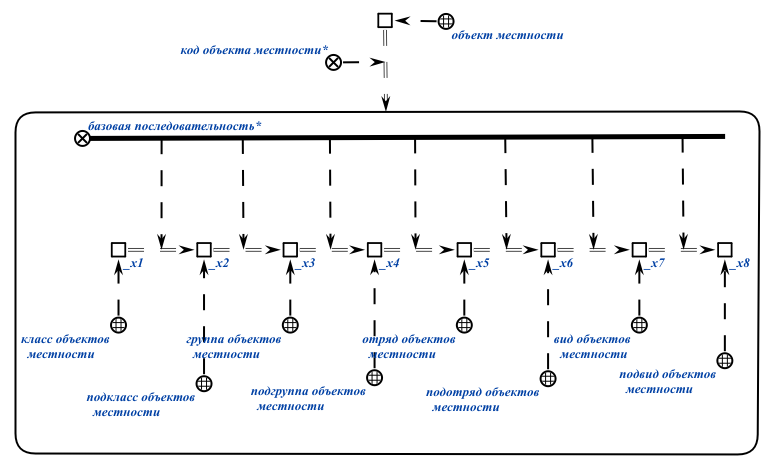
\includegraphics[scale=0.8]{author/part7/figures/geo_code.png}
	\label{fig:pic1}
\end{figure}

Для каждого \textit{объекта местности} выделены основные, присущие только ему, семантические характеристики. Особо отметим, что метрические характеристики таким свойством не обладают.  
Согласно данному классификатору каждый класс \textit{объектов местности} имеет уникальное однозначное обозначение. Иерархия классификатора имеет восемь ступеней классификации и состоит из \textit{кода класса}, \textit{кода подкласса}, \textit{кода группы}, \textit{кода подгруппы}, \textit{кода отряда}, \textit{кода подотряда}, \textit{кода вида}, \textit{кода подвида}. Таким образом, благодаря способу кодирования уже заданы родовидовые связи, отражающие соотношения различных классов \textit{объектов местности}, а также установлены характеристики конкретного класса \textit{объектов местности}. В связи с тем, что задаются основные свойства и отношения не конкретных \textit{физических объектов}, а их классов, то такая информация является по отношению к конкретным \textit{объектам местности} метаинформацией, а совокупность данной метаинформации представляет собой онтологию \textit{объектов местности}, которая в свою очередь является частью \textit{базы знаний} \textit{интеллектуальной геоинформационной системы}.

\begin{SCn}	
	\scnheader{объект местности}
	\scnrelfrom{разбиение}{\textbf{\textit{Типология объектов местности по локализации}}\scnsupergroupsign}
	\begin{scnindent}
		\begin{scneqtoset}
			\scnitem{точечный объект местности}
			\begin{scnindent}
				\scnidtf{объект местности, который не выражается в масштабе карты}
				\begin{scnrelfromlist}{пример;включение}
					\scnitem{колодец}
					\scnitem{осветительная опора}
					\scnitem{дорожный знак}
				\end{scnrelfromlist}
			\end{scnindent}
			\scnitem{линейный объект местности}
			\begin{scnindent}
				\scnidtf{объект местности, длина которого выражается в масштабе карты}
				\begin{scnrelfromlist}{пример;включение}
					\scnitem{мост}
				\end{scnrelfromlist}
			\end{scnindent}
			\scnitem{полилинейный объект местности}
			\begin{scnindent}
				\scnidtf{объект местности, состоящий из двух и более сегментов линейных объектов}
				\begin{scnrelfromlist}{пример;включение}
					\scnitem{река}
					\scnitem{дорога}
					\scnitem{улица}
				\end{scnrelfromlist}
			\end{scnindent}
			\scnitem{площадной объект местности}
			\begin{scnindent}
				\scnidtf{объект местности, площадь которого выражается в масштабе карты}
				\begin{scnrelfromlist}{пример;включение}
					\scnitem{озеро}
					\scnitem{административный район}
					\scnitem{государство}
				\end{scnrelfromlist}
			\end{scnindent}
		\end{scneqtoset}
	\end{scnindent}
\end{SCn}

\subsection{Геосемантические характеристики объектов местности}
\label{chapter_gis_sec_geo_elements}

Особенностью \textit{геоонтологии} является использование для формализации \textit{предметных областей} специальных элементов, уточняющих пространственные характеристики объектов местности, которые назовем \textbf{\textit{геосемантическими характеристиками объектов местности}}.

\begin{SCn}
\scnheader{геосемантическая характеристика объекта местности}
\begin{scnrelfromset}{разбиение}
	\scnitem{координатное местоположение объекта местности\scnsupergroupsign}
	\scnitem{пространственное отношение}
	\scnitem{пространственное отношение главных направлений}
	\scnitem{динамика состояния объекта местности\scnsupergroupsign}
\end{scnrelfromset}
\end{SCn}

\begin{SCn}
\scnheader{координатное местоположение объекта местности}
\scnidtf{географическое положение, расположение \textit{объекта местности} или явления, которое задается в \textit{системе геодезических координат}}

\scnheader{геокодирование}
\scnidtf{установление связи между \textit{объектом местности} и его \textit{местоположением}}
\scnsubset{действие}
\end{SCn}

\begin{SCn}
\scnheader{пространственное отношение}
\scnidtf{класс отношений, задающие семантические свойства объекта местности по отношению к другим объектам местности}
\begin{scnrelfromset}{разбиение}
	\scnitem{топологическое пространственное отношение}
	\scnitem{отношение пространственной упорядоченности}
	\scnitem{метрическое пространственное отношение}
\end{scnrelfromset}
\end{SCn}

\begin{SCn}
\scnheader{отношение пространственной упорядоченности}
\begin{scnrelfromset}{разбиение}
	\scnitem{отношение расположения объектов местности}
	\scnitem{отношение главных направлений объектов местности}
\end{scnrelfromset}
\end{SCn}

\begin{SCn}
\scnheader{отношение расположения объектов местности}
\scnsubset{ориентированное отношение}
\scnidtf{позволяет определить, какое положение занимает один \textit{объект местности} по отношению к другому \textit{объекту местности}}
\scnhaselement{объект местности располагается перед другим объектом местности*}
\scnhaselement{объект местности располагается за другим объектом местности*}
\scnhaselement{объект местности располагается слева от другого объекта местности*}
\begin{scnindent}
	\scnhaselementrole{пример}{Водонапорная башня располагается слева от дороги}
\end{scnindent}
\scnhaselement{объект местности располагается справа от другого объекта местности*}
\scnhaselement{объект местности располагается над другим объектом местности*}
\scnhaselement{объект местности располагается под другим объектом местности*}
\scnhaselement{объект местности располагается ближе другого объекта местности*}
\scnhaselement{объект местности располагается дальше другого объекта местности*}
\end{SCn}

\begin{SCn}
\scnheader{отношение главных направлений объектов местности}
\scnsubset{ориентированное отношение}
\scnidtf{позволяет определить, какое главное направление занимает один \textit{объект местности} по отношению к другому \textit{объекту местности}}
\scntext{примечание}{\textit{отношение главных направлений объектов местности} инвариантно относительно сдвига и масштабирования}
\scnhaselement{объект местности по отношению к другому объекту местности занимает главное направление север*}
\scnhaselement{объект местности по отношению к другому объекту местности занимает главное направление северо-восток*}
\scnhaselement{объект местности по отношению к другому объекту местности занимает главное направление восток*}
\scnhaselement{объект местности по отношению к другому объекту местности занимает главное направление юго-восток*}
\scnhaselement{объект местности по отношению к другому объекту местности занимает главное направление юг*}
\scnhaselement{объект местности по отношению к другому объекту местности занимает главное направление юг-запад*}
\scnhaselement{объект местности по отношению к другому объекту местности занимает главное направление запад*}
\scnhaselement{объект местности по отношению к другому объекту местности занимает главное направление северо-запад*}
\end{SCn}

\begin{SCn}
\scnheader{метрическое пространственное отношение}
\scnidtf{характеризует информацию о расстоянии между \textit{объектами местности}}
\scnrelfrom{измерение}{километр}
\scnrelfrom{измерение}{метр}
\scnsuperset{шкальное метрическое пространственное отношение}
\begin{scnindent}
	\scnrelfrom{измерение}{шкала}
\end{scnindent}
\end{SCn}

\begin{SCn}
\scnheader{система геодезических координат}
\scnidtf{система координат, используемая для определения местоположения объектов на Земле}
\scnhaselementrole{пример}{WGS84}
\begin{scnindent}
	\scntext{примечание}{Всемирная система геодезических параметров Земли 1984 года, в число которых входит система геоцентрических координат. В отличие от локальных систем, является единой системой для всей планеты.}
\end{scnindent}
\scnhaselementrole{пример}{СК-63}
\scnhaselementrole{пример}{СК-95}
\end{SCn}

\subsection{Топологические пространственные отношения между объектами местности}
\label{chapter_gis_sec_relations}

Между экземплярами \textit{объектов местности} можно установить \textit{топологические пространственные отношения}: \textit{включение*}, \textit{граничить*}, \textit{пересечение*} и \textit{примыкание*}. 

\begin{SCn}
\scnheader{топологическое пространственное отношение}
\scnidtf{класс \textit{пространственных отношений}, заданных над \textit{объектами местности}, находящихся в отношении связности и смежности между \textit{объектами местности}}
\scnrelfrom{примечание}{\textit{топологическое пространственное отношение} инвариантно относительно перемещения, поворота и масштабирования}
\scnhaselement{включение*}
\begin{scnindent}
	\scnsuperset{включение точечного объекта местности в площадной объект местности*}
	\begin{scnindent}
		\scnrelfrom{пример}{\includegraphics[scale=1.0]{author/part7/figures/point\_to\_square\_inclusion.png}}
	\end{scnindent}
	\scnsuperset{включение линейного (полилинейного) объекта местности в площадной объект местности*}
	\begin{scnindent}
		\scnrelfrom{пример}{\includegraphics[scale=1.0]{author/part7/figures/linear\_to\_square\_inclusion.png}}
	\end{scnindent}
	\scnsuperset{включение площадного объекта местности в площадной объект местности*}
	\begin{scnindent}
		\scnrelfrom{пример}{\includegraphics[scale=1.0]{author/part7/figures/square\_to\_square\_inclusion.png}}
	\end{scnindent}
\end{scnindent}
\scnhaselement{граничить*}
\begin{scnindent}
	\scnrelfrom{пример}{\includegraphics[scale=1.0]{author/part7/figures/square\_to\_square\_edgion.png}}
\end{scnindent}
\scnhaselement{пересечение*}
\begin{scnindent}
	\scnsuperset{пересечение двух линейных (полинейных) объектов местности*}
	\begin{scnindent}
		\scnrelfrom{пример}{\includegraphics[scale=1.0]{author/part7/figures/linear\_linear\_intersection.png}}
	\end{scnindent}
	\scnsuperset{пересечение линейного (полинейного) и площадного объектов местности*}
	\begin{scnindent}
		\scnrelfrom{пример}{\includegraphics[scale=1.0]{author/part7/figures/linear\_square\_intersection.png}}
	\end{scnindent}
\end{scnindent}
\scnhaselement{примыкание*}
\begin{scnindent}
	\scnrelfrom{пример}{\includegraphics[scale=1.0]{author/part7/figures/linear\_to\_linear\_contiguition.png}}
\end{scnindent}
\end{SCn}

Отношение \scnqqi{включения*} будет устанавливаться между \textit{площадным} и \textit{линейным}, \textit{площадным} и \textit{точечным}, \textit{площадными объектами местности}. Отношение \scnqqi{пересечения*} будет устанавливаться между \textit{линейными} и \textit{площадными} и \textit{линейными объектами местности}. Отношение \scnqqi{граничить*} будет устанавливаться между \textit{площадными объектами местности}. Отношение \scnqqi{примыкания*} устанавливается между \textit{линейными объектами местности}. Для всех \textit{картографических отношений} существуют структуры для их хранения.

\subsection{Стратифицированная модель информационного пространства объектов местности}
\label{chapter_gis_sec_strat_model}

С целью \textit{интеграции} \textit{предметных областей} с пространственными компонентами \textit{геоинформационных систем}, соответственно повышения \textit{интероперабельности} этих систем, предлагается \textit{Стратифицированная модель информационного пространства объектов местности}, которая задается следующим образом:

\begin{equation} 
\label{<eq2_1>} 
S^{\mu}, \mu  \in I = \{S_{PO\mu}, S_{OM}, E_{OM}\},
\end{equation} 

\parindent=8mm
\noindent \hangindent=22mm \hangafter=1
где $I$ - множество \textit{предметных областей};

\hangindent=22mm \hangafter=1
$S_{PO\mu}$ --- онтология ${\mu}$-ой \textit{предметной области};

\hangindent=30mm \hangafter=1
$S_{OM}$ --- онтология \textit{объектов местности};

\hangindent=30mm \hangafter=1
$E_{OM}$ --- экземпляры \textit{объектов местности}.
\parindent=0mm

На \textit{\nameref{fig:pic2_1}} представлена геометрическая интерпретация предложенной \textit{гибридной модели знаний}, где показано, что слой экземпляров \textit{объектов местности} является интегрирующим слоем с предметными знаниями различных \textit{предметных областей}, в которых уже непосредственно используются конкретные \textit{объекты местности}. При такой организации знаний возможно многократно использовать  разработанную онтологию \textit{объектов местности} в разных предметных областях и, соответственно, для решения различных прикладных задач.

\begin{figure}[H]
	\caption{Рисунок. Стратифицированная модель информационного пространства объектов местности}
	\includegraphics[width=\linewidth]{author/part7/figures/gis\_knowledge\_model.JPG}
	\label{fig:pic2_1}
\end{figure}

\section{Решатель задач интеллектуальной геоинформационной ostis-системы}
\label{chapter_gis_ps}

\textbf{\textit{решатель задач интеллектуальной геоинформационной ostis-системы}} представляет собой коллектив взаимодействующих друг с другом \textit{sc-агентов}, позволяющих решать \textit{геоинформационные задачи}. Ниже приведена базовая декомпозиция \textit{решателя задач интеллектуальной геоинформационной системы} на основные классы sc-агентов геоинформационного назначения.

\begin{SCn}
	\scnheader{решатель задач интеллектуальной геоинформационной системы}
	\begin{scnrelfromset}{декомпозиция}
		\scnitem{Абстрактный sc-агент вычисления геометрических характеристик объектов местности}
		\begin{scnindent}
			\begin{scnrelfromset}{декомпозиция}
				\scnitem{Абстрактный sc-агент обработки точечных объектов местности}
				\scnitem{Абстрактный sc-агент обработки линейных (полилинейных) объектов местности}
				\scnitem{Абстрактный sc-агент обработки площадных объектов местности}
			\end{scnrelfromset}
		\end{scnindent}
		\scnitem{Абстрактный sc-агент определения типа локализации объекта местности}
		\scnitem{Абстрактный sc-агент сопряжения с различными картографическими системами и сервисами, системами измерений и временными интервалами}
		\begin{scnindent}
			\begin{scnrelfromset}{декомпозиция}
				\scnitem{Абстрактный sc-агент сопряжения с картографическими системами}
				\scnitem{Абстрактный sc-агент сопряжения с единицами измерений}
				\scnitem{Абстрактный sc-агент сопряжения с временными интервалами}
			\end{scnrelfromset}
		\end{scnindent}
		\scnitem{Абстрактный sc-агент установления топологических связей между объектами местности}
		\scnitem{Абстрактный sc-агент верификации базы знаний объектов местности}
		\begin{scnindent}
			\begin{scnrelfromset}{декомпозиция}
				\scnitem{Абстрактный sc-агент верификации полноты заполнения базы знаний объектов местности}
				\scnitem{Абстрактный sc-агент верификации корректности значений семантических атрибутов объектов местности}
				\scnitem{Абстрактный sc-агент верификации корректности значений пространственных атрибутов объектов местности}
			\end{scnrelfromset}
		\end{scnindent}
	\end{scnrelfromset}
\end{SCn}

\section{Картографический интерфейс интеллектуальной геоинформационной ostis-системы}
\label{chapter_gis_sec_map_specification}

\textbf{\textit{картографический интерфейс}} --- это \textit{пользовательский интерфейс}, предназначенний для визуального отображения \textit{объектов местности} на каком-то \textit{языке карт}.
\textit{картографический интерфейс} как вид \textit{пользовательского интерфейса} должен обладать следующими свойствами:
\begin{textitemize}
	\item высоким уровнем согласованности понятий, используемых при визуализации информации об объектах местности;
	\item высоким уровнем простоты (естественностью) и понятности для любого конечного пользователя (интерфейс должен быть снисходительным к уровню подготовки пользователя, то есть дружелюбным);
	\item высоким уровнем привлекательности (естетичности) и легкости восприятия;
	\item и так далее.
\end{textitemize}

Частным видом \textit{картографического интерфейса} является \textit{картографический интерфейс интеллектуальной геоинформационной ostis-системы}.

Разрабатываемый \textit{Язык карт для ostis-систем} относится к семейству семантически совместимых языков --- \textit{sc-языков} и предназначен для формального описания \textit{объектов местности} и отношений между ними в \textit{геоинформационных системах}. Поэтому \textbf{\textit{Синтаксис Языка карт для ostis-систем}}, как и \textit{синтаксис} любого другого \textit{sc-языка}, является \textit{Синтаксисом SC-кода}. Такой подход позволяет:
\begin{textitemize}
\item использовать минимум средств для интерпретации заданных \textit{объектов местности} на карте;
\item использовать \textit{Язык вопросов для ostis-систем};
\item сводить поиск на большую часть заданных \textit{вопросов} к поиску информации в текущем состоянии \textit{базы знаний ostis-системы}.
\end{textitemize}

\textbf{\textit{Денотационная семантика Языка карт для ostis-систем}} включает \textit{пространственные отношения} и \textit{геосемантические характеристики объектов местности}.

\begin{SCn}
\scnheader{Язык карт для ostis-систем}
\scnidtf{Предлагаемый нами вариант внешнего языка для представления и визуализации информации об объектах местности в картографическом интерфейсе интеллектуальной геоинформационной ostis-системы}
\scniselement{sc-язык}
\scnrelfrom{синтаксис языка}{Синтаксис Язык карт для ostis-систем}
\begin{scnindent}
	\scnsubset{Синтаксис SC-кода}
\end{scnindent}
\scnrelfrom{денотационная семантика языка}{Денотационная семантика Языка карт для ostis-систем}
\begin{scnindent}
	\scnidtf{Онтологии объектов местности, пространственных отношений между ними и их геосемантических характеристик}
	\scnsuperset{Семантическая классификация вопросов}
\end{scnindent}
\scnrelfrom{операционная семантика языка}{Операционная семантика Языка карт для ostis-систем}
\begin{scnindent}
	\scnidtf{Коллектив sc-агентов интерпретации Языка карт для ostis-систем}
\end{scnindent}
\end{SCn}

Ключевое достоинство \textit{картографического интерфейса интеллектуальной геоинформационной ostis-системы} и соответствующего ему \textit{Языка карт для ostis-систем} по сравнению с другими видами \textit{пользовательских интерфейсов} состоит в том, что с помощью их можно визуализировать любые \textit{классы объектов местности\scnsupergroupsign} и информацию о них достаточно простым способом, понятным любому пользователю.

Покажем пример отображения \textit{семантической окрестности} \textit{объекта местности} \scnqqi{Река Березина} на \textit{SCg-коде} (\textit{\nameref{fig:gis_map_berezina_scg_format}}) и \textit{Языке карт} (\textit{\nameref{fig:gis_map_berezina_map_format}}).

\begin{figure}[H]
	\caption{Рисунок. Описание Реки Березина на SCg-коде}
	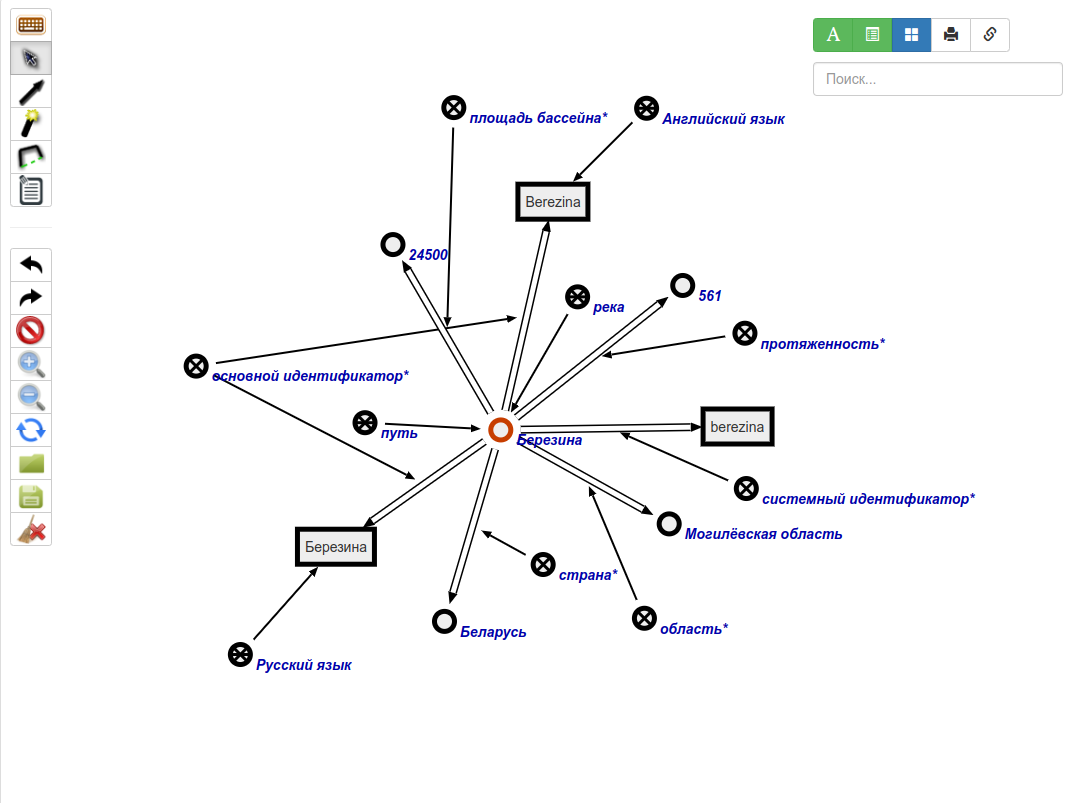
\includegraphics[scale=0.45]{author/part7/figures/berezina.png}
	\label{fig:gis_map_berezina_scg_format}
\end{figure}

\begin{figure}[H]
	\caption{Рисунок. Описание Реки Березина на Языке карт}
	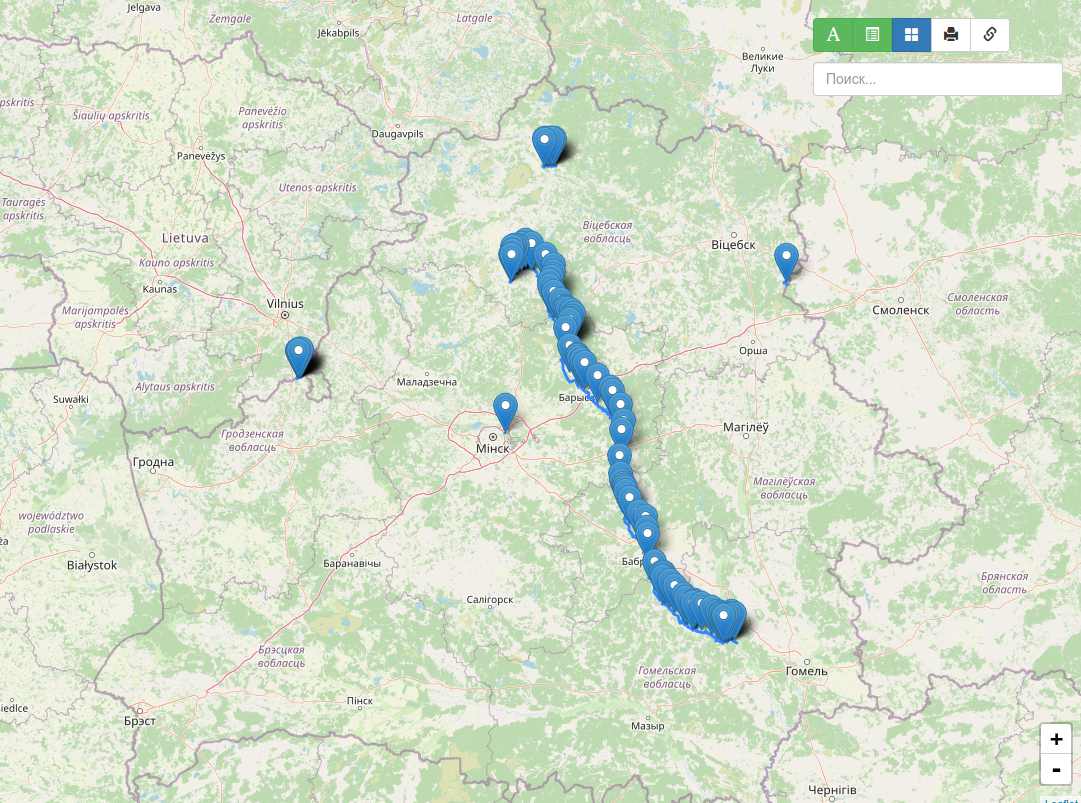
\includegraphics[scale=0.45]{author/part7/figures/berezina_map.png}
	\label{fig:gis_map_berezina_map_format}
\end{figure}

На обоих рисунках показаны \textit{семантические окрестности} одного и того же \textit{объекта местности}, но представленных на разных \textit{внешних языках представления знаний}: \textit{SCg-коде} и \textit{SCg-коде}.

Отображение информации об \textit{объекте местности} происходит при помощи средств \textit{Метасистемы OSTIS} (см. \textit{Главу \ref{chapter_ims_standard}~\nameref{chapter_ims_standard}}) и  \textit{Технологии OpenMapStreet} и включает следующие этапы:
\begin{textitemize}
	\item поиск \textit{семантической окрестности} заданного \textit{объекта местности} (то есть \textit{пространственных отношений} между заданным \textit{объектом местности} и другими \textit{объектами местности}, а также геосемантических характеристик заданного \textit{объекта местности});
	\item определение географических кодов \textit{территориальных объектов местности}, в которых располагается заданный \textit{объект местности}, а также других объектов местности, связанных \textit{пространственными отношениями} с заданным \textit{объектом местности};
	\item получение картографических данных о \textit{территориальных объектах местности} и их соотнесение с информацией о \textit{территориальных объектах местности} в базе знаний;
	\item определение класса \textit{объекта местности};
	\item визуализация \textit{семантической окрестности} заданного \textit{объекта местности} на \textit{Языке карт}.
\end{textitemize}

\section{Многократно используемые компоненты интеллектуальных геоинформационных ostis-систем}
\label{chapter_gis_sec_mic_components}

Одним из требованием, предъявляемым к \textit{Технологии проектирования интеллектуальных геоинформационных систем}, является обеспечение возможности совместного использования в рамках \textit{интеллектуальных геоинформационных ostis-систем} различных \textit{видов знаний} и различных \textit{моделей решения задач}, а также различных видов \textit{интерфейсов}. Следствием данного требования является необходимость реализации компонентного подхода на всех уровнях, от простых компонентов баз знаний, решателей задач и интерфейсов до целых \textit{встраиваемых ostis-систем} (см. \textit{\ref{reusable_component_section}~\nameref{reusable_component_section}}).

Таким образом, \textit{база знаний интеллектуальной геоинформационной ostis-системы} должна включать спецификацию \textit{объектов местности}, то есть описание их \textit{семантических окрестностей} (см. \textit{\nameref{fig:gis_kb_component}}), \textit{решатель задач интеллектуальной геоинформационной ostis-системы} --- спецификацию sc-агентов, решающих различные \textit{геоинформационные задачи} (например, sc-агент классификации \textit{географических объектов} (см. \textit{\nameref{fig:gis_ps_component}}), sc-агент определения \textit{пространственных отношений} между \textit{объектами местности} и так далее), а \textit{картографический интерфейс интеллектуальной геоинформационной ostis-системы} --- описание \textit{отношений} между \textit{объектами местности} на \textit{карте}.

\begin{figure}[H]
	\caption{SCg-текст. Пример многократно используемого компонента базы знаний интеллектуальных геоинформационных ostis-систем}
	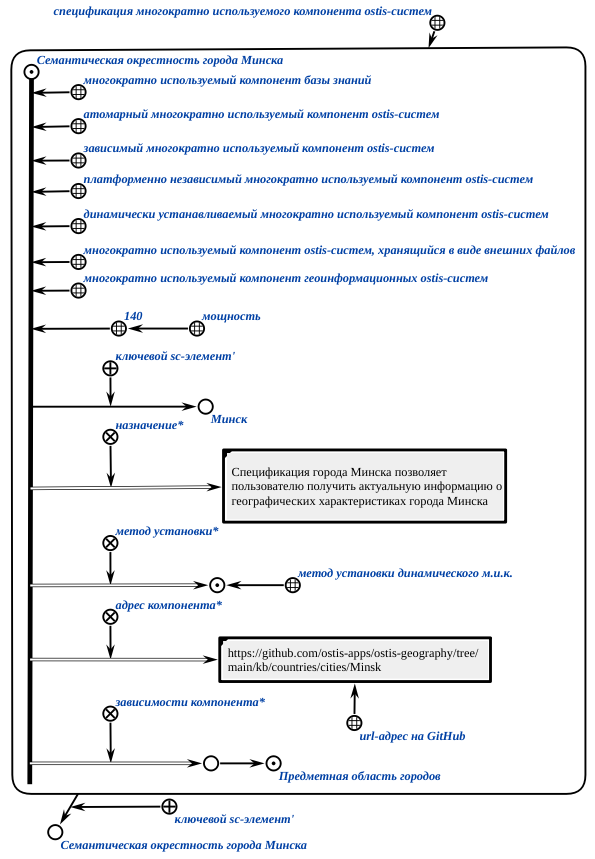
\includegraphics[scale=0.8]{author/part7/figures/gis_kb_component.png}
	\label{fig:gis_kb_component}
\end{figure}

\begin{figure}[H]
	\caption{SCg-текст. Пример многократно используемого компонента решателя задач интеллектуальных геоинформационных ostis-систем}
	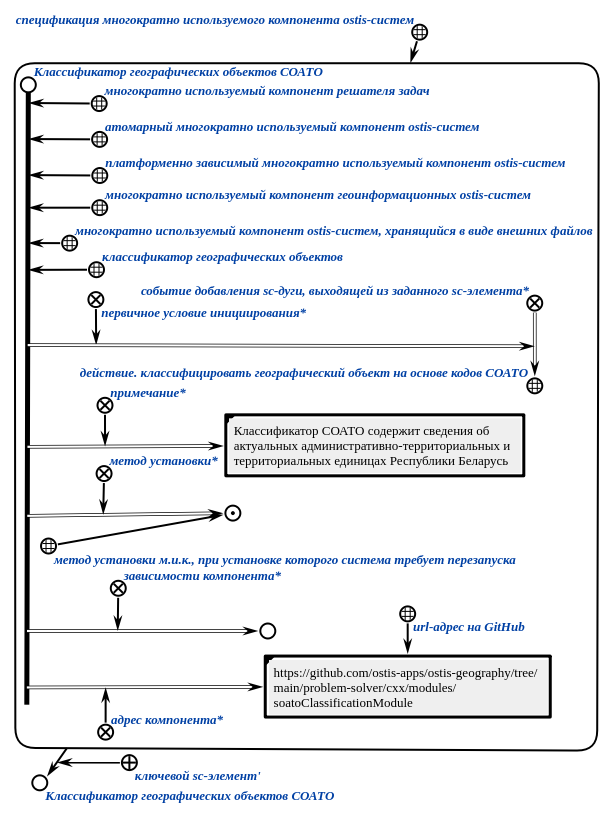
\includegraphics[scale=0.8]{author/part7/figures/gis_ps_component.png}
	\label{fig:gis_ps_component}
\end{figure}

\section{Средства автоматизации проектирования интеллектуальных геоинформационных ostis-систем}
\label{chapter_gis_sec_automatization}

Проектирование \textit{интеллектуальных геоинформационных систем} осуществляется поэтапно. На первом этапе формируется \textit{база знаний} \textit{предметной области} и с этой целью анализируется электронная карта и осуществляется трансляция в \textit{базу знаний} \textit{объектов местности} с установлением \textit{геосемантических характеристик объектов местности} для соответствующей территории. На данном этапе определяется, во-первых, к какому классу принадлежит исследуемый \textit{объект местности} и, далее в зависимости от типа объекта, формируется \textit{понятие} \textit{базы знаний}, соответствующее конкретному \textit{объекту местности}. Таким образом, создается множество понятий, описывающих конкретные \textit{объекты местности} для каждого \textit{класса объектов местности\scnsupergroupsign}. Следует отметить, что именно на данном этапе формирования \textit{базы знаний} устанавливаются \textit{геосемантические характеристики объектов местности}.

На втором этапе проектирования \textit{интеллектуальной геоинформационной системы} происходит интеграция полученной на первом этапе \textit{базы знаний} с внешними \textit{базами знаний}. На этом этапе, помимо географических \textit{знаний}, добавляться \textit{знания} смежных \textit{предметных областей}, тем самым становится возможным установление межпредметных связей. Наглядным примером служит интеграция с биологическими классификаторами, которые в реализации представляют собой онтологию объектов флоры и фауны. Такая интеграция расширяет функциональные и интеллектуальные возможности прикладной \textit{интеллектуальной геоинформационной системы}. Отметим, что на данном этапе снимается омонимия в названиях \textit{объектов местности}, принадлежащих классам населенных пунктов. Для населенных пунктов \textit{Республики Беларусь} это достигается за счет использования \textit{системы обозначений объектов административно-территориального деления и населенных пунктов} и осуществляется семантическое сопоставление \textit{объектов местности} по следующему принципу:
\begin{textitemize}
	\item определяется \textit{класс объекта местности\scnsupergroupsign};
	\item определяется подкласс, вид, подвид \textit{объекта местности} в соответствии с классификатором \textit{объектов местности}, то есть виды \textit{объектов местности} в \textit{геоонтологии};
	\item определяются атрибуты и характеристики, которые присущи данному \textit{классу объектов местности\scnsupergroupsign};
	\item определяются значения характеристик для данного \textit{класса объекта местности\scnsupergroupsign};
	\item устраняется омонимия идентификации;
	\item устанавливаются соответствующие связи между \textit{объектом местности} и \textit{понятием} в \textit{базе знаний} с установленными \textit{геосемантическими характеристиками объектов местности};
	\item устанавливаются \textit{пространственные отношения} между \textit{объектами местности}, отнесенными к определенным классам.
\end{textitemize}

\begin{figure}[H]
	\caption{Рисунок. Этапы проектирования баз знаний интеллектуальных геоинформационных ostis-систем}
	\includegraphics[width=\linewidth]{author/part7/figures/gis\_design\_steps.png}
	\label{fig:gis_design_steps}
\end{figure}

\section*{Заключение к Главе \ref{chapter_gis}}

Перечислим основные положения данной главы:
\begin{textitemize}
	\item развитие \textit{геоинформационных систем} заключается в их интеллектуализации, благодаря чему расширяется круг прикладных задач с использованием \textit{знаний} об \textit{объектах местности};   
	\item предложено карту рассматривать как \textit{информационную конструкцию}, элементами которой являются \textit{объекты местности}, тем самым обеспечивается \textit{интероперабельность} \textit{геоинформационных систем} за счет перехода от карты к семантическому описанию элементов карты, то есть объектов местности и связей (пространственных отношений) между ними;
	\item обеспечение \textit{интероперабельности} достигается благодаря разработке онтологий предметных областей, а установление \textit{геосемантических характеристик объектов местности} позволяет задавать пространственные характеристики \textit{объектов местности}; 
	\item наличие частной \textit{Технологии проектирования интеллектуальных геоинформационных систем} обеспечивает процесс проектирования интеллектуальных геоинформационных систем, построенных по принципам ostis-систем.
\end{textitemize}